In diesem Kapitel wird eine Auswahl relevanter Experimente aus \cite{book:regele} beschrieben. Der Aufbau der Experimente wird durch Abbildungen und assistierend durch Text wiedergegeben. Auf den Abbildungen sind statische Hindernisse grau, freie Zellen weiß, die Startpositionen der Agenten blau und die Zielpositionen grün markiert. Die Experimente teilen sich in zwei Kapitel auf. Das erste Kapitel \ref{chap:allgemein} beschreibt jene Experimente, für die keine Messwerte vorliegen und Kapitel \ref{chap:mitMesswerten} diejenigen, für die Messwerte dokumentiert sind.

Für die Experimente sind die Agenten wie in \cite{book:regele} konfiguriert. Die Parameter werden folgend wiederholt.

Die Enfernungskarten, der Agenten, umfassen immer die gesamte Karte eines Experiments. Für jeden Bewegungsschritt führt ein Agent genau einen Berechnungsschritt durch. Ein Agent ist etwas kleiner als eine Zelle. Die Konfiguration für die Prioritätsangleichung ist wie folgt:\newline
\(BasePrio=0\), \(PrioNoBlock=1\), \(PrioBlock=10\) und \(PrioFullBlock=19\). Ein Prioritätsüberlauf, im Falle einer ungelösten Verklemmung, tritt erst ab einem Wert von \(PrioMax=400\) auf. Wenn ein solcher Überlauf eintritt, setzt sich der Prioritätswert auf eine zufällige Zahl zwischen null und zehn zurück. Jedes Experiment wird 30 Mal wiederholt. 
Der Durchmesser \((d)\) der Umgebungskarte variiert. Bei Experimenten mit Karten die 30 Felder breit sind, ist \(d=21\). Für die Experimente mit Messwerten beträgt \(d=13\). Für die anderen Experimente gilt \(d=9\). Die zeitliche Berechnungstiefe ist abhängig von der Dimension der Umgebungskarte und wird folgendermaßen bestimmt \(t\textsubscript{max}=0.75*d\).

Sofern nicht anders gekennzeichnet, sind \cite{book:regele} als Quelle für den Aufbau der Experimente, die Messwerte und die zu erwartenden Beobachtungen anzunehmen.

In den folgenden Unterkapiteln wird häufiger von Gruppen die Rede sein. Im Kontext des CoDy Algorithmus sind damit keine logisch zusammenhängenden Agenten gemeint. Eine Gruppe bezeichnet hier lediglich Agenten, die in Nähe zueinander starten.

\section{Allgemeine Experimente}
\label{chap:allgemein}
Für die folgenden Experimente liegen keine Messwerte vor. Sie eignen sich aber, dank der Tatsache, dass bestimmte Verhaltensmuster erwartet werden, zum Überprüfen, ob der CoDy Algorithmus richtig implementiert wurde.

Für jedes Experiment wird zuerst geklärt, was mit diesem gezeigt werden soll. Darauf folgend wird der Aufbau des Experiments beschrieben und die zu erwartenden Beobachtungen vorgestellt. Abschließend werden, für alle Experimente zusammenfassend, die eigenen Beobachtungen vorgestellt.

Für alle Experimente dieses Kapitel gilt die Erwartungshaltung, dass alle 30 Durchläufe erfolgreich absolviert werden.

%
\subsection{Kurze Engstelle}
\label{chap:engstelle}
Mit diesem Experiment wird gezeigt, dass Agenten Ausweichbewegungen durchführen und Wartephasen einlegen, um andere Agenten passieren zu lassen.

\textbf{Aufbau des Experiments}
\begin{figure}[H]
    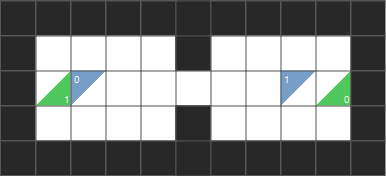
\includegraphics[height=40mm]{images/one_slit.png}
    \centering
    \caption{Aufbau für das Durchfahren zweier Agenten durch eine kurze Engstelle}
    \label{fig:engstelle}
\end{figure}
Die Karte misst neun mal drei Felder. In der Mitte der Karte ist eine eins mal eins Feld breite Engstelle. Auf beiden Seiten dieser Engstelle stehen sich Agenten gegenüber, die die Engstelle durchfahren müssen, um ihre Zielposition zu erreichen.

\textbf{Erwartete Beobachtungen}\newline
Der Agent, der zuerst einen Weg plant, fährt direkt auf seine Zielposition. Der andere Agent fährt eine Ausweichposition in der unmittelbaren Nähe der Engstelle an. Nachdem der erste Agent die Engstelle passiert hat, wird sich der zweite Agent auf direkten Weg zu seinem Ziel machen.
%
\subsection{Umweg}
\label{chap:umweg}
Hier wird gezeigt wie ein Agent einen anderen verdrängt, aber auch das Agenten Umwege in Kauf nehmen.

\textbf{Aufbau des Experiments}
\begin{figure}[H]
    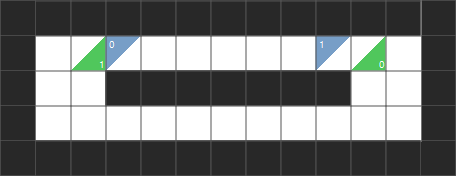
\includegraphics[height=40mm]{images/detour.png}
    \centering
    \caption{Aufbau für ein Szenario, in dem ein Agent einen Umweg in Kauf nimmt}
    \label{fig:umweg}
\end{figure}
Die Karte in Abbildung \ref{fig:umweg} misst elf mal drei Felder und wird mittig, horizontal durch einen Streifen aus sieben Feldern getrennt. Die Start- und Zielpositionen der Agenten sind so angeordnet, dass die nördliche Engstelle den kürzeren Weg darstellt und die südliche Engstelle den Umweg.

\textbf{Erwartete Beobachtungen}\newline
Für kleine Umgebungskarten, also solche bei denen sich die Umgebungskarten der beiden Agenten erst nach dem Annähern überlappen, werden sich beide Agenten in der nördlichen Engstelle annähern. Wenn sich die Umgebungskarten dann überlappen, wird einer der Agenten den Zuschlag erhalten und den anderen Agenten verdrängen. Dieser wird dann über die südliche Engstelle, also über den Umweg, sein Ziel anfahren.

Für größere Umgebungskarten wird der Agent, der zuerst seinen Weg plant, direkt und der andere über den Umweg sein Ziel anfahren.
%
\subsection{Tunnel}
\label{chap:tunnel}
Dieses Experiment testet, wie anfällig die Agenten für Verklemmungen sind.

\textbf{Aufbau des Experiments}
\begin{figure}[H]
    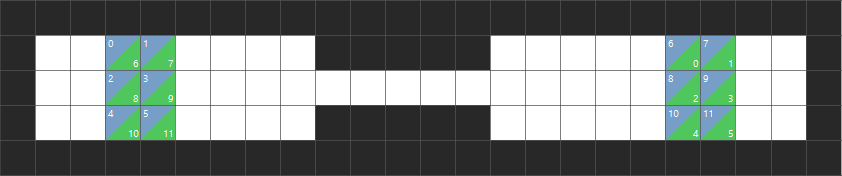
\includegraphics[width=\textwidth]{images/tunnel_2_groups.png}
    \centering
    \caption{Ausgangssituation für das Durchqueren eines Tunnels von zwei Gruppen, bestehend aus jeweils sechs Agenten}
    \label{fig:tunnel}
\end{figure}
In diesem Experiment durchqueren zwei Gruppen aus jeweils sechs Agenten eine Engstelle, die fünf Felder lang und ein Feld breit ist. Jeder Agent muss die Engstelle passieren um sein Ziel zu erreichen.

\textbf{Erwartete Beobachtungen}\newline
Im ersten Schritt nähern sich beide Gruppen der Engstelle. Während eine Gruppe anfängt die Engstelle zu durchqueren, fahren die Agenten der anderen Gruppe Ausweichpositionen an und verlängern damit die Engstelle. Im Laufe des Experiments wechseln die Gruppen ihre Rollen häufiger.
%
\subsection{Tunnel mit kleiner Ausweichbucht}
\label{chap:ausweichbucht}
Dieses Experiment dient zur Veranschaulichung der dynamischen Prioritäten. Diese Situation kann, dezentral, nämlich nicht durch feste Prioritäten gelöst werden.

\textbf{Aufbau des Experiments}
\begin{figure}[H]
    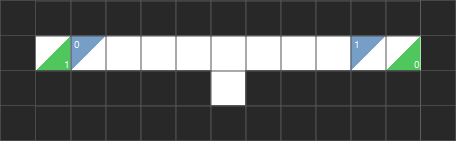
\includegraphics[height=32mm]{images/tunnel_turnout.png}
    \centering
    \caption{Aufbau für die Vorbeifahrt zweier Agenten in einem Tunnel mit einer kleinen Ausweichbucht}
    \label{fig:ausweichbucht}
\end{figure}
Zwei sich gegenüberstehende Agenten versuchen, in einer elf Felder langen und ein Feld schmalen Engstelle aneinander vorbei auf ihre Zielpositionen zu fahren. Der Tunnel hat in der Mitte ein zusätzliches freies Feld, das von den Agenten genutzt werden muss, um aneinander vorbei zu fahren.

\textbf{Erwartete Beobachtungen}\newline
Zuerst werden die beiden Agenten aufeinander zu fahren. Dann wird einer der beiden Agenten zurückgedrängt werden. Wenn der zurückgedrängte Agent sich nicht weiter zurückdrängen lässt, wird dieser seine Priorität erhöhen und den zu erst drängenden Agenten in die Ausweichbucht drängen, was dann beiden Agenten ermöglicht aneinander vorbei zu ihren Zielpositionen zu fahren. Es kann auch passieren, dass ein Agent die Ausweichbucht direkt anfährt und es zu keiner Verdrängung kommt.
%
\subsection{Durchfahren einer stehenden Menge}
\label{chap:menge}
In diesem Experiment wird gezeigt, dass obwohl ein Agent sein Ziel schon erreicht hat, immer noch aktiv an der passiven Kooperation teilnimmt.

\textbf{Aufbau des Experiments}
\begin{figure}[H]
    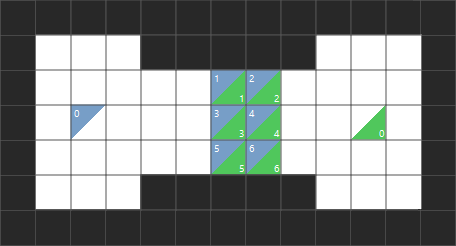
\includegraphics[height=56mm]{images/crowd_drive-through.png}
    \centering
    \caption{Aufbau für das Durchfahren eines Agenten durch ein Menge stehender Agenten}
    \label{fig:menge}
\end{figure}
Die Abbildung \ref{fig:menge} zeigt die Karte für dieses Experiment. Diese hat Dimensionen von elf mal fünf Felder. In der Mitte ist eine fünf Felder lange und drei Felder breite Engstelle. In dieser Engstelle stehen in zwei Reihen hintereinander sechs Agenten. Die Startpositionen dieser Agenten sind gleichzeitig ihre Zielpositionen. Ein weiterer Agent hat seine Startposition auf der linken Seite der Engstelle und seine Zielposition auf der Rechten. Er muss also durch die stehende Menge, um sein Ziel zu erreichen.

\textbf{Erwartete Beobachtungen}\newline
Die Agenten "'3"' und "'4"' werden von Agent "'0"' verdrängt, fahren also von ihren Zielpositionen weg, um Platz für Agent "'0"' zu machen. Es ist auch möglich, dass dabei andere Agenten von ihren Zielpositionen verdrängt werden. Nachdem Agent "'0"' die Menge durchquert hat, fahren alle Agenten wieder zurück zu ihren Zielpositionen.
%
\subsection{Kreuzung}
\label{chap:kreuzung}
Dieses Szenario dient der Beobachtung der Flexibilität der Agenten. Außerdem soll der Unterschied zu einem zentralen Ansatz deutlich gemacht werden und die Skalierbarkeit des Ansatzes gezeigt werden.

\textbf{Aufbau des Experiments}
\begin{figure}[H]
    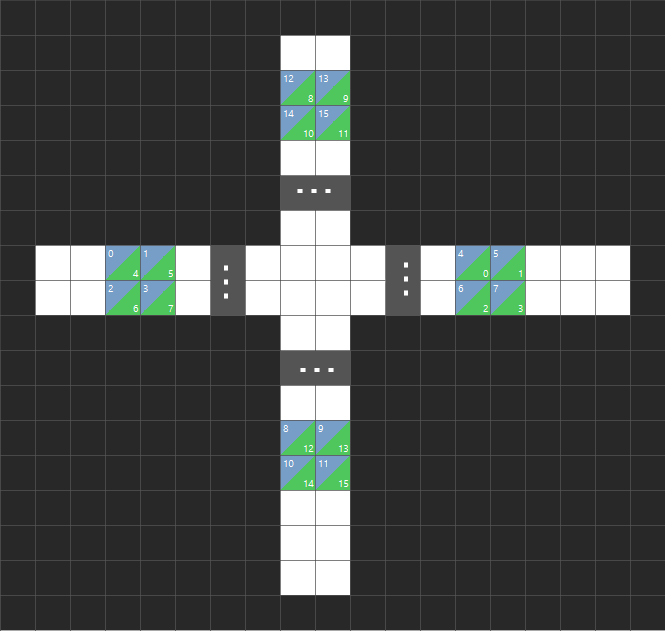
\includegraphics[width=\textwidth]{images/junction.png}
    \centering
    \caption{Aufbau für das Passieren einer Kreuzung von vier Gruppen, bestehend aus jeweils vier Agenten}
    \label{fig:kreuzung}
\end{figure}
In diesem Experiment versuchen vier Gruppen von jeweils vier Agenten eine Kreuzung zu durchqueren. Ziel jeder Gruppe ist es, die gegenüberliegende Seite in gleicher Formation zu erreichen. Der Kreuzungsbereich besteht aus acht freien Feldern, bietet also nicht genügend Platz für alle Agenten. Normale Verkehrsregeln, zum Beispiel das Rechtsfahrgebot, Vorfahrtsregeln oder das Bilden von Fahrspuren, sind keine Lösungen, die ein konfliktfreies aneinander Vorbeifahren der Agenten ermöglichen. Die vier Fahrbahnen der Kreuzung sind jeweils zwei Felder breit und 14 Felder lang.

\textbf{Erwartete Beobachtungen}\newline
Wegen der dynamischem Prioritäten ist eine Vielzahl an Lösungen zu beobachten. Der Berechnungsaufwand pro Agent steigt, trotz der gestiegenen Teilnehmerzahl, nicht.
Ein möglicher zentraler Ansatz würde vermutlich zwei Gruppen blockieren und die übrigen gegenüberliegenden Gruppen durch die Kreuzung passieren lassen, um erst danach den blockierten Gruppen die Durchfahrt zu gewähren. Dies ist vergleichbar mit einer Ampel an einer Kreuzung im Straßenverkehr.


%
\subsection{Beobachtungen}
\label{chap:beobachtungen}
Alle zu erwartenden Beobachtungen konnten, so wie in \cite{book:regele} beschrieben, in den eigens ausgeführten Experimenten beobachtet werden.

\section{Experimente mit Messwerten}
\label{chap:mitMesswerten}
Die folgenden Experimente wurden zum Überprüfen der Leistungsfähigkeit des Algorithmus entwickelt. Im Kern stehen sich immer zwei gleich große Gruppen von Agenten gegenüber, deren Ziel es ist die Startpositionen der Agenten der anderen Gruppen zu erreichen. Die Anzahl der Agenten variiert zwischen den Experimenten und der freie Raum wird tendenziell immer kleiner. Für jedes Experiment ist es das Ziel, dass in allen 30 Wiederholung eine Lösung gefunden wird, also alle Agenten ihr Ziel erreichen.

Der Aufbau der Experimente und das zu erwartende Verhalten der Agenten werden vorgestellt. Im Kapitel \ref{chap:ergebnisse} folgen dann die Messwerte aus \cite{book:regele} und die eigenen.

\subsection{Sechs gegen sechs: Lockere Vorbeifahrt}
\label{chap:6x6_locker}
Das erste Experiment dieser Reihe bietet vergleichsweise viel Platz. Es ist vor allem für den späteren Vergleich interessant.

\textbf{Aufbau des Experiments}
\begin{figure}[H]
    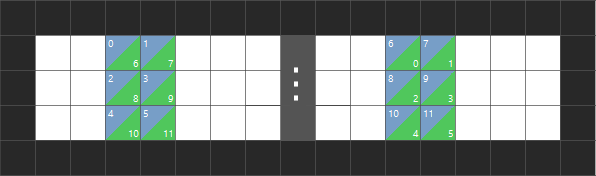
\includegraphics[width=\textwidth]{images/6vs6_spacy.png}
    \centering
    \caption{Aufbau für die lockere Vorbeifahrt zweier Gruppen, bestehend aus jeweils sechs Agenten}
    \label{fig:6x6Locker}
\end{figure}
 Die Abbildung \ref{fig:6x6Locker} zeigt eine Karte die drei mal 30 Felder misst. Es stehen sich zwei Gruppen, bestehend aus jeweils sechs Agenten, gegenüber. Zum rechten beziehungsweise linken Rand sind für die Gruppen noch ein paar freie Felder vorhanden. Damit soll es den Agenten möglich sein, Ausweichbewegungen nach hinten hin ausführen zu können.
\subsection{Sechs gegen sechs: Enge Vorbeifahrt}
\label{chap:6x6_eng}
In diesem Experiment ist der Platz für Bewegungen sehr beschränkt. Zwölf Felder sind von Agenten belegt und lediglich neun sind frei. 

\textbf{Aufbau des Experiments}
\begin{figure}[H]
    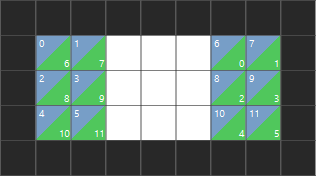
\includegraphics[height=40mm]{images/6vs6_tight.png}
    \centering
    \caption{Aufbau für die enge Vorbeifahrt zweier Gruppen, bestehend aus jeweils sechs Agenten}
    \label{fig:6x6Eng}
\end{figure}
Die Karte für dieses Experiment ist sieben mal drei Felder groß. Es stehen sich zwei Gruppen aus jeweils sechs Agenten gegenüber. Wie in Abbildung \ref{fig:6x6Eng} zu erkennen, befindet sich zwischen den beiden Gruppen ein Block aus drei mal drei freien Feldern.
\subsection{Drei gegen drei: Enge Vorbeifahrt}
\label{chap:3x3_eng}
Dieses Experiment dient als Vergleich zum Vorangegangenen. Die Auswirkung die die Anzahl der Roboter hat, soll hiermit untersucht werden. 

\textbf{Aufbau des Experiments}
\begin{figure}[H]
    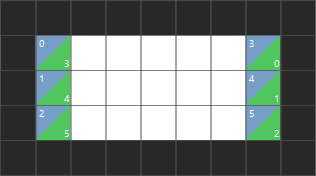
\includegraphics[height=40mm]{images/3vs3.png}
    \centering
    \caption{Aufbau für die enge Vorbeifahrt zweier Gruppen, bestehend aus jeweils drei Agenten}
    \label{fig:3x3}
\end{figure}
Die Karte für dieses Experiment ist sieben mal drei Felder groß. Es stehen sich zwei Gruppen aus jeweils drei Agenten gegenüber. Wie in Abbildung \ref{fig:3x3} zu erkennen, befindet sich zwischen den beiden Gruppen ein Block aus fünf mal drei freien Feldern.
\subsection{Vier gegen vier: Enge Vorbeifahrt}
\label{chap:4x4_eng}
Dieses Experiment schränkt den Platz der Agenten weiter ein. Die Zahl der belegten Felder ist hier größer als die Anzahl der freien Felder. Besonders für dieses Experiment ist, dass ein Graph vorliegt der die Prioritätswerte der Agenten über die Zeit zeigt (siehe Abbildung \ref{tab:resultsCoDy} und \ref{tab:myResults}). 

\textbf{Aufbau des Experiments}
\begin{figure}[H]
    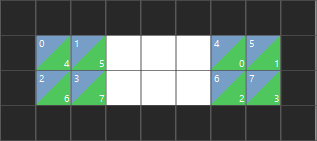
\includegraphics[height=32mm]{images/4vs4_tight.png}
    \centering
    \caption{Aufbau für die enge Vorbeifahrt zweier Gruppen, bestehend aus jeweils vier Agenten}
    \label{fig:4x4}
\end{figure}
Die Karte für dieses Experiment misst sieben mal zwei Felder. Acht Agenten teilen sich in zwei gleich große Gruppen und stehen sich gegenüber.
\subsection{Messergebnisse}
\label{chap:ergebnisse}
\begin{table}[H]
    \centering
    \begin{tabular}{c|c|c|c|c|c|c}
       \textbf{Experiment} & \textbf{Gelöst} & \textbf{Prioritäts-Überlauf}
        & \(\textbf{s\textsubscript{opt}}\) & \(\textbf{s\textsubscript{CoDy}}\)
        & \(\textbf{t\textsubscript{opt}}\) & \(\textbf{t\textsubscript{CoDy}}\)\\ \hline
       \textbf{6-vs-6-locker} & 30 von 30 & 0 von 30
       & 19.5 & 20.97 & 22 & 24.33 \\ \hline
       \textbf{6-vs-6-eng} & 26 von 30 & 1 von 30
       & 5.45 & 11.5 & 10.35 & 21.89 \\ \hline
       \textbf{3-vs-3-eng} & 30 von 30 & 3 von 30
       & 5.5 & 6.35 & 6.33 & 7.68 \\ \hline
       \textbf{4-vs-4-eng} & 27 von 30 & 4 von 30
       & 5 & 10.85 & 10.5 & 24.96
    \end{tabular}
    \caption{Messwerte der Experimente aus \cite{book:regele}}
    \label{tab:resultsCoDy}
\end{table}

\begin{table}[H]
    \centering
    \begin{tabular}{c|c|c|c|c}
       \textbf{Experiment} & \textbf{Gelöst} & \textbf{Prioritäts-Überlauf}
        & [\textbf{\(\bar{s}\textsubscript{u}\)}, \textbf{\(\bar{s}\textsubscript{o}\)}]
        & [\textbf{\(\bar{t}\textsubscript{u}\)}, \textbf{\(\bar{t}\textsubscript{o}\)}]\\ \hline
       \textbf{6-vs-6-locker} & 30 von 30 & 0 von 30 & [20.01, 22.33] & [23.92, 26.4]\\ \hline
       \textbf{6-vs-6-eng} & 18 von 30 & 18 von 18 & [8.78, 9.81] & [19.52, 23.09]\\ \hline
       \textbf{3-vs-3-eng} & 27 von 30 & 0 von 27 & [7.3, 7.58] & [9.53, 9.97]\\ \hline
       \textbf{4-vs-4-eng} & 20 von 30 & 20 von 20 & [13.72, 25.2] & [23.04, 41.04]
    \end{tabular}
    \caption{Messwerte der selbst durchgeführten Experimente}
    \label{tab:myResults}
\end{table}

Die eigenen Messwerte weichen teils stark von den vorgegeben Messwerten ab. Lediglich das Experiment "'\ref{chap:6x6_locker} Sechs gegen sechs: Lockere Vorbeifahrt"' trifft die Erwartungen.

Für die eigenen Messungen ist anzumerken, dass für den Prioritätsüberlauf nicht immer "'von 30"' angegeben ist. Das hat damit zu tun, dass die Simulationsumgebung nur Daten erzeugt, wenn ein Experiment erfolgreich war.

\begin{figure}[H]
    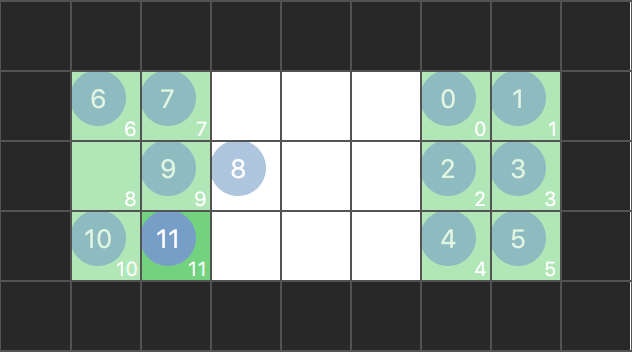
\includegraphics[height=40mm]{images/6vs6_tight_full_block.png}
    \centering
    \caption{Beispielhafte Totalblockade für das Experiment "'\ref{chap:6x6_eng} Sechs gegen sechs: Enge Vorbeifahrt"'}
    \label{fig:6x6EngFullBlock}
\end{figure}
Für das Experiment "'\ref{chap:6x6_eng} Sechs gegen sechs: Enge Vorbeifahrt"' ist der zurückgelegte Strecke etwas besser als erwartet. Der Zeitbedarf trifft die Erwartung. Auffällig ist jedoch, dass nur 18 statt 26 Wiederholungen erfolgreich sind und es in allen, statt nur bei einer Wiederholung, zu Prioritätsüberläufen kam. Bei den zwölf ungelösten Wiederholungen ist eine Variation der in Abbildung \ref{fig:6x6EngFullBlock} gezeigten Situation eingetreten. 

Die Werte für "'\ref{chap:3x3_eng} Drei gegen drei: Enge Vorbeifahrt"'
weichen nur leicht von den erwarteten ab. Statt 30 werden nur 27 Wiederholungen gelöst. Dafür kommt es in den gelösten Wiederholungen aber nicht zu Prioritätsüberläufen. Die drei erwarteten Wiederholungen, die einen Prioritätsüberläufen haben, entstehen aus Situationen, in denen sich die Agenten in breiter Front aufeinander zu bewegen. In den eigenen Experimenten führten genau diese Situation zu den drei ungelösten Wiederholungen.

Die gemessenen Werte weichen für das Experiment "'\ref{chap:4x4_eng} Vier gegen vier: Enge Vorbeifahrt"' am stärksten ab. Es werden nur in 20 statt 27 Wiederholungen Lösungen gefunden. In jeder Wiederholung kommt es zu Prioritätsüberläufen. Auch das war nicht erwartet. Die Konfidenzintervalle für die durchschnittlich zurückgelegte Strecke und den durchschnittlichen Zeitbedarf sind im Vergleich besonders groß. Die erwartete Strecke ist nicht mal im Intervall enthalten. Wie Abbildungen \ref{fig:4x4_prio_2} deutlich zeigt, wird der erwartete Prioritätsverlauf verfehlt. Statt das die Priorität der Agenten über die Zeit stetig ansteigt und teilweise wieder zurückgeht, pendeln bei den eigenen Experimenten die Prioritätswerte zwischen minimalen und maximalen Werten hin und her.

\begin{figure}[H]
    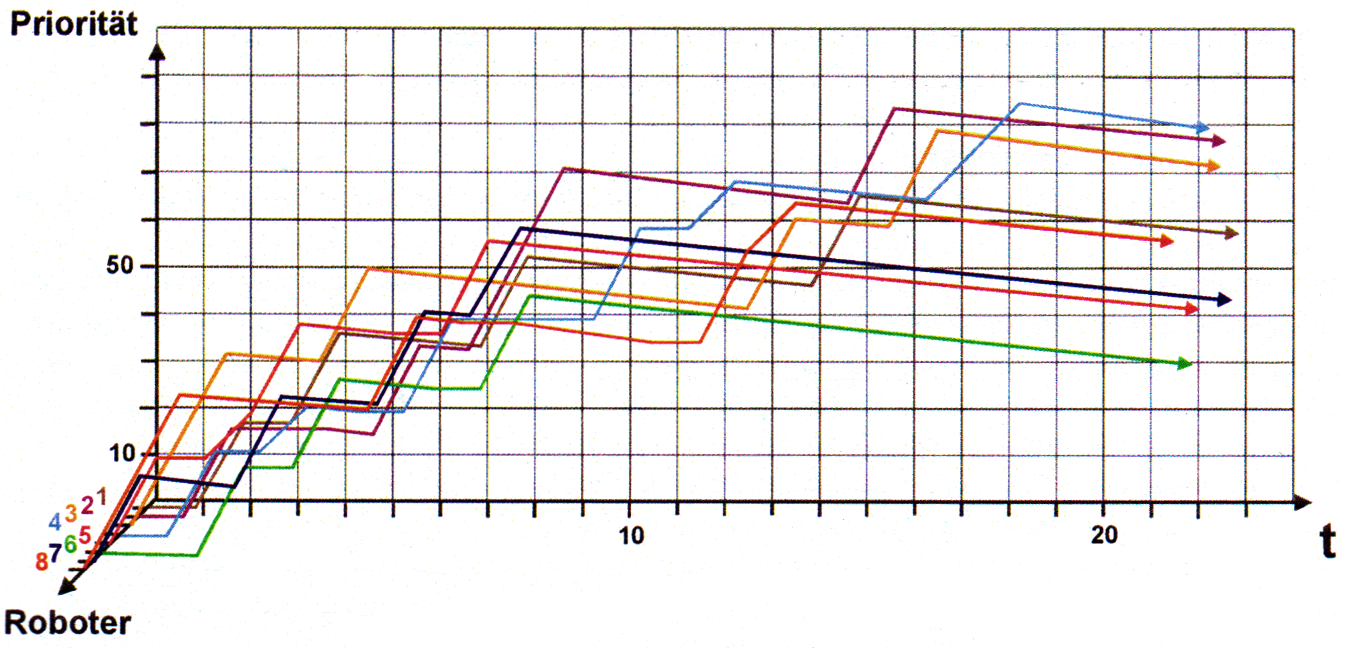
\includegraphics[width=\textwidth]{images/4vs4_tight_prio_ref.png}
    \centering
    \caption{Prioritätsverlauf aller Agenten für das Experiment "'\ref{chap:4x4_eng} Vier gegen vier: Enge Vorbeifahrt"' aus \cite{book:regele}}
    \label{fig:4x4_prio_1}
\end{figure}

\begin{figure}[H]
    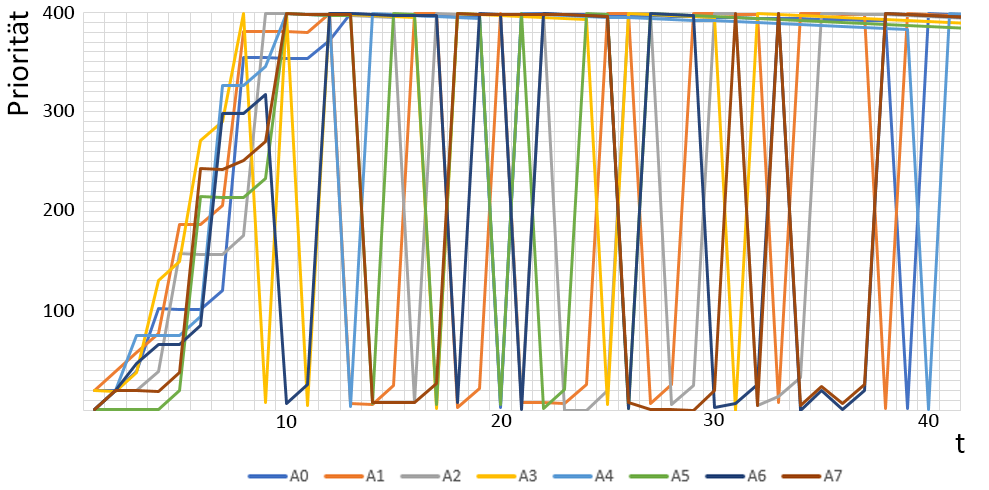
\includegraphics[width=\textwidth]{images/4vs4_tight_prio.png}
    \centering
    \caption{Prioritätsverlauf aller Agenten für das Experiment "'\ref{chap:4x4_eng} Vier gegen vier: Enge Vorbeifahrt"' der selbst durchgeführten Experimente}
    \label{fig:4x4_prio_2}
\end{figure}